% ============================================================
%  Appendix
% ============================================================

\section{Implementation Details}
\label{app:impl}

\paragraph{Algorithm.}
Algorithm~\ref{alg:main} gives the full \sysname{} evolution procedure described in
Section~\ref{sec:method_loop}.

\begin{algorithm}[h]
\SetAlgoLined
\KwIn{$\mathcal{D}_{\text{train}}$, frozen VLM $\pi_\theta$, iterations $N$, candidates $M$}
\KwOut{Capability set $\mathcal{C} = (\mathcal{S}, \mathcal{T})$}
$\mathcal{C} \leftarrow (\emptyset, \emptyset)$\;
\For{$n = 1$ \KwTo $N$}{
  Solve $\mathcal{D}_{\text{train}}$ with $f_{\mathcal{C}}$; collect attempts\;
  $\mathcal{D}_{\text{sub}} \leftarrow$ sample from $\mathcal{D}_{\text{train}}$\;
  $a, r \leftarrow \textsc{AnalyzerDecider}(\mathcal{D}_{\text{sub}};\, \pi_\theta)$\;
  $\{(s_m, t_m)\}_{m=1}^{M} \leftarrow \textsc{Generator}(a, r;\, \pi_\theta)$\tcp*{$s_m$ paired with $t_m$ acts as its mastery SOP}
  $m^\star \leftarrow \arg\max_{m} \mathrm{Acc}\bigl(f_{\mathcal{C} \cup (s_m, t_m)};\, \mathcal{D}_{\text{train}}\bigr)$\;
  \If{accuracy improves}{
    $\mathcal{C} \leftarrow \mathcal{C} \cup \{(s_{m^\star}, t_{m^\star})\}$\;
  }
}
\Return{$\mathcal{C}$}\;
\caption{\sysname{} evolution loop.}
\label{alg:main}
\end{algorithm}

\paragraph{Role prompts.}
\sysname{} uses three role-specific system prompts for the same base VLM:
\textit{Solver} (standard QA prompt with capability context injected),
\textit{AnalyzerDecider} (root-cause analysis and decision), and
\textit{Generator} (skill or tool generation).
All prompts are provided in full at \url{[anonymised repository]}.

\paragraph{Skill retrieval.}
At inference time, the Solver retrieves the top-$K{=}3$ skills from $\mathcal{S}$ using BM25
cosine similarity over skill titles and When-to-Use fields.
Retrieved skill text is appended to the system prompt.

\paragraph{Tool invocation.}
The Solver inspects each tool's mastery SOP to decide whether to invoke it on the current input.
If the input matches a tool's supported patterns, the tool is applied and its output image(s)
are appended to the multimodal context.
Tool execution is sandboxed with a 30-second timeout and resource limits.

\paragraph{Hyperparameters.}
Table~\ref{tab:hyperparams} lists all hyperparameter settings.

\begin{table}[h]
\centering
\footnotesize
\setlength{\tabcolsep}{3pt}
\caption{Hyperparameter settings.}
\label{tab:hyperparams}
\begin{tabular}{@{}>{\raggedright\arraybackslash}p{0.28\columnwidth}
                >{\raggedright\arraybackslash}p{0.16\columnwidth}
                >{\raggedright\arraybackslash}p{0.44\columnwidth}@{}}
\toprule
\textbf{Parameter} & \textbf{Value} & \textbf{Description} \\
\midrule
$k$         & 200        & Training cases per benchmark \\
$N$         & 3          & Evolution iterations \\
$K$         & 3          & Skills retrieved per query \\
Max tool lines & 150     & Max lines for generated Python tool \\
Mastery sample & 50      & Cases for mastery profiling \\
Regression buffer & 20   & Cases for tool regression test \\
Temperature & 0.7        & Generator temperature \\
Max tokens (gen.) & 2048 & Max tokens for capability generation \\
\bottomrule
\end{tabular}
\end{table}

\paragraph{Compute.}
Experiments use the frozen VLM backbones listed in Section~\ref{sec:setup}.
Total API calls per benchmark: $\leq k \times N \times 3 = 1{,}800$ calls
(solver + analyzer + generator, upper bound).
Estimated token usage: $\sim$3M tokens per benchmark.
No GPU training is performed.

\section{Mechanism Ablations}
\label{app:ablation_mechanisms}

Experiment~I in the main paper already isolates the contribution of each capability
\emph{type}: the \emph{None}, \emph{Skill Only}, \emph{Tool Only}, and \emph{Full} rows of
Table~\ref{tab:evolution_full} answer whether skills, tools, or both account for the
observed gains. The ablations here test a complementary question: when the Full system is
used, which \emph{mechanisms} inside the evolution loop (Section~\ref{sec:method_loop}) are
doing the work? Each variant removes one design decision and holds the rest fixed, so each
row of Table~\ref{tab:ablation_mechanism} rules out one alternative explanation for the
Full system's gains.

\paragraph{Setup.}
All variants use the same protocol as Experiment~I (frozen GPT-5.4 backbone; 20\% of each
benchmark's training split as $\mathcal{D}_{\text{train}}$; $N{=}3$ evolution iterations;
$M$ candidate skill$+$tool combinations per iteration) and rebuild $\mathcal{C}$ from
scratch so any deficit reflects the ablated mechanism rather than a carried-over artifact.
The two primary benchmarks are \textbf{ChartQA} (cognitive / procedural) and
\textbf{HRBench} (perceptual / high-resolution); \textbf{MathVista} and \textbf{V$^\star$}
are reported as secondary checks.

\paragraph{Main mechanism table.}
Table~\ref{tab:ablation_mechanism} reports six ablation variants spanning the four
mechanism families: diagnosis (whether the AnalyzerDecider sees correct cases and visual
input), exploration (multi-candidate generation), inference-time gating (paired mastery
skill), and persistence (cross-case library). The Full row reproduces the Full entry from
Table~\ref{tab:evolution_full} for reference.

\begin{table*}[t]
\centering
\small
\setlength{\tabcolsep}{4pt}
\renewcommand{\arraystretch}{1.18}
\begin{tabular}{lp{0.34\textwidth}cccc}
\toprule
\textbf{Variant} & \textbf{Ablated mechanism}
  & \textbf{ChartQA} & \textbf{HRBench}
  & \textbf{MathVista} & \textbf{V$^\star$} \\
\midrule
Full \sysname{}              & --- (full evolution loop)
  & & & & \\
\midrule
Generic Skill                & evolved library $\to$ hand-neutral task prompt
  & & & & \\
Failure-Only Diagnosis       & AnalyzerDecider sees only incorrect cases
  & & & & \\
Text-only Diagnosis          & AnalyzerDecider sees no images or tool artefacts
  & & & & \\
Single-Candidate ($M{=}1$)   & one Generator proposal per iteration; no selection
  & & & & \\
No Paired Mastery Skill      & tool emitted without its paired skill (action $=$ both)
  & & & & \\
No Persistence               & capabilities not stored across cases
  & & & & \\
\bottomrule
\end{tabular}
\caption{%
  \textbf{Mechanism ablations.}
  Each row removes one mechanism from \sysname{} while holding the rest fixed
  (GPT-5.4; 20\% training split; $N{=}3$). The Full row reproduces the Full entry from
  Table~\ref{tab:evolution_full}. Numbers will be filled in once the corresponding runs
  complete.
}
\label{tab:ablation_mechanism}
\end{table*}

\subsection{Generic Skill vs. Evolved Capability}
\label{app:abl_generic}

\paragraph{What is removed.}
The evolved capability library is replaced with a single hand-neutral task prompt that
gives generic task advice (for ChartQA: ``read the chart carefully, identify relevant
values, reason step by step''; for HRBench: ``inspect local details before answering and
verify the target object''). No diagnosis, generation, validation, or persistence is run.

\paragraph{What this rules out.}
A pure prompt-engineering account would predict that Generic Skill closes most of the gap
to Full, since the evolved skills are themselves natural-language SOPs. If Generic Skill
improves over Direct by only a small margin and stays well below Full, the gap is
attributable to mechanism-level evolution---failure-specific procedures, applicability
triggers, and pitfalls that a generic prompt cannot anticipate---rather than to the
presence of any task-aware prompt.

\subsection{Failure-Only Diagnosis}
\label{app:abl_failure_only}

\paragraph{What is removed.}
The AnalyzerDecider only sees the incorrect cases in the sampled sub-training set; the
correct cases are dropped. Everything else---multimodal input, multi-candidate
exploration, paired mastery skill, persistence---is unchanged.

\paragraph{What this rules out.}
Most prior self-improvement work treats correct cases as nothing to learn from. This
variant tests that assumption directly. If Failure-Only Diagnosis matches Full, then the
correct cases carry no useful diagnostic signal and the abstract's framing of ``diagnoses
both correct and incorrect attempts'' is decorative. A gap supports the design choice:
correct attempts tell the AnalyzerDecider \emph{which sub-patterns the current
$\mathcal{C}$ already handles}, which sharpens the next capability proposal toward what is
still missing.

\subsection{Text-only Diagnosis}
\label{app:abl_textonly}

\paragraph{What is removed.}
The AnalyzerDecider's inputs are restricted to text only: the question, the agent's answer
(correct or incorrect), the ground-truth answer, and the reasoning trace. No original
image, no intermediate tool output, and no processed visual artefact is passed in.

\paragraph{What this rules out.}
Text reflection can say \emph{that} an answer was wrong, but it cannot tell whether a
crop was misaligned, whether a zoomed region missed the target, or whether a processed
image introduced artefacts. We expect the gap to Full to be largest on the perceptual
benchmarks (HRBench, V$^\star$). On ChartQA the gap should be smaller because many
failures there are procedural; a small ChartQA gap with a large HRBench/V$^\star$ gap is
itself the signature of the visual-diagnosis claim.

\subsection{Single-Candidate ($M{=}1$)}
\label{app:abl_single_candidate}

\paragraph{What is removed.}
The Generator produces a single capability proposal per iteration (the same setting as
typical generate-then-validate tool-creation methods such as
CREATOR~\citep{DBLP:conf/emnlp/QianH0Q0J23} and LATM~\citep{DBLP:conf/iclr/Cai00CZ24}). The validate-and-promote
step (Eq.~\ref{eq:selection}) collapses to a binary accept/reject of that single
candidate against the training set.

\paragraph{What this rules out.}
A reviewer might ask whether the multi-candidate $\arg\max$ in Eq.~\ref{eq:selection} is
load-bearing or whether the first proposal is usually good enough. If Single-Candidate
roughly matches Full, the exploration step is decorative. A measurable gap shows that
diverse candidates plus selection by training-set accuracy is what turns a noisy proposal
distribution into a reliably improving library.

\subsection{No Paired Mastery Skill}
\label{app:abl_mastery}

\paragraph{What is removed.}
When the AnalyzerDecider's action is \texttt{both}, the Generator emits only the tool and
not its paired mastery skill. The tool is added to $\mathcal{T}$ but has no
$\textsc{When-to-Use}$ predicate gating its invocation at inference, so any skill
retrieval that surfaces a tool reference exposes the tool unconditionally.

\paragraph{What this rules out.}
Prior tool-creation methods deploy generated tools indiscriminately. The paired-skill
design in Section~\ref{sec:method_mastery} predicts that gating tool invocation by
retrieval of an applicability-encoding skill is what keeps tool usage selective.
No Paired Mastery Skill is expected to keep or even increase tool-usage rate but reduce
accuracy on benchmarks where naive tool exposure can hurt---MathVista is the canonical
cautionary case.

\subsection{No Persistence}
\label{app:abl_persistence}

\paragraph{What is removed.}
Capabilities promoted during one iteration are not stored in $\mathcal{C}$. The agent can
still reflect on a case and immediately retry it with the generated capability, but the
capability is discarded before the next case is processed, so no cross-case retrieval
occurs.

\paragraph{What this rules out.}
A retry-only account would predict that most of Full's gain comes from in-place retry on
the triggering case rather than from cross-case reuse. If No Persistence matches Full on
held-out accuracy, the library is a bookkeeping device with no inferential value. A gap
shows that the system's advantage comes from accumulating capabilities that future cases
can retrieve, not just from one more attempt at the triggering case. ChartQA is the
cleanest test because failures there form recurring families (stacked-bar boundary
reading, multi-series selection) that a single capability can fix across many held-out
cases.

\subsection{Sensitivity to Training Subset Size and Iteration Count}
\label{app:abl_sensitivity}

The main paper fixes the training subset at 20\% of each benchmark's training split and
runs $N{=}3$ evolution iterations. A sensitivity sweep over smaller fractions (e.g.\ 5\%,
10\%) and over $N \in \{1, 3, 5\}$ tests how quickly the library saturates: a small subset
should already expose the most frequent procedural / perceptual patterns, with diminishing
returns as the subset grows; $N{=}1$ should miss capabilities that only surface after
earlier ones reshape the trajectory, while $N{=}3$ and $N{=}5$ should produce comparable
libraries. We treat this as a robustness check rather than a tuning study; the operating
point is chosen to fit the per-benchmark budget.

\subsection{Summary}
\label{app:abl_summary}

Read together, the six mechanism ablations are designed to triangulate the same claim
from six different angles. Generic Skill rules out a pure prompt-engineering explanation;
Failure-Only Diagnosis rules out ``correct cases carry no signal''; Text-only Diagnosis
rules out ``text reflection is enough'' and supports the visual-diagnosis channel;
Single-Candidate rules out ``the first proposal is good enough'' and supports
multi-candidate exploration; No Paired Mastery Skill rules out ``expose every generated
tool'' and supports applicability-bounded deployment; and No Persistence rules out
``per-case retry is enough'' and supports cross-case capability accumulation. The
expected pattern is that removing any one mechanism reduces held-out accuracy noticeably,
but no single ablation collapses the system---consistent with the design view that the
six mechanisms implement complementary aspects of capability evolution rather than
redundant copies of the same underlying lever.

\paragraph{Practical diagnostic.}
The mechanism ablations also suggest a practical rule of thumb for new task families. If
the bottleneck is procedural---visual evidence is present but the reasoning is weak---skill
evolution is the lower-cost first choice; if a different view of the image is required
before the evidence becomes accessible, tool evolution is necessary. A practitioner
targeting a new benchmark can use a small pilot run (e.g.\ 5\% of the training split with
$N{=}1$) to inspect which kinds of capabilities are generated and whether they transfer
beyond the triggering examples.

\section{Additional Results}
\label{app:results}

\subsection{Training Set Size Sensitivity}

\begin{figure}[ht]
\centering
\fbox{\rule{0pt}{3cm}\rule{0.7\columnwidth}{0pt}}
\caption{Placeholder for ChartQA accuracy vs.\ training set size
$k \in \{10, 25, 50, 100, 200\}$ at $N{=}3$ iterations.}
\label{fig:k_sensitivity}
\end{figure}

Figure~\ref{fig:k_sensitivity} shows ChartQA accuracy as a function of training set size
$k \in \{10, 25, 50, 100, 200\}$ at $N{=}3$ iterations.

\subsection{Per-Category Analysis on ChartQA}

% TODO: Insert breakdown of accuracy gains by chart type (bar, line, pie, scatter).

\subsection{Distribution-Shift Adaptation: Time Series and Aggregates}
\label{app:distribution_shift_timeseries}

Figure~\ref{fig:distribution_shift} in the main paper aggregates the distribution-shift
experiment across backbones and stream constructions. This appendix shows the per-step
trajectory along the stream (Figure~\ref{fig:distribution_shift_timeseries}) and the
full per-backbone numerical aggregates (Table~\ref{tab:distribution_shift}).

\begin{figure}[ht]
  \centering
  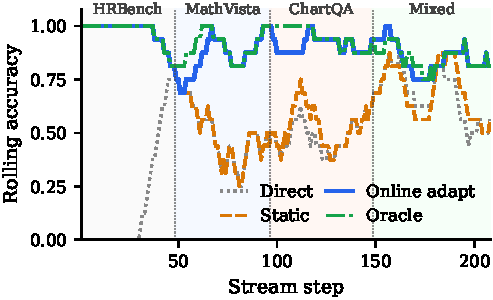
\includegraphics[width=\columnwidth]{figures/distribution_shift_timeseries.pdf}
  \caption{%
    \textbf{Rolling accuracy along the natural stream (GPT-5.4).}
    Phase labels above the plot mark the newly introduced family at each shift; earlier
    families remain present in the mix. \emph{Static} lags at each shift; \emph{Online
    adapt} catches up to \emph{Oracle} within a 2--7 case detection latency.
  }
  \label{fig:distribution_shift_timeseries}
\end{figure}

\begin{table}[ht]
\centering
\small
\setlength{\tabcolsep}{4pt}
\renewcommand{\arraystretch}{1.12}
\resizebox{\columnwidth}{!}{%
\begin{tabular}{lcccc}
\toprule
\textbf{Replay protocol}
  & \textbf{Direct}
  & \textbf{Static}
  & \textbf{Online adapt}
  & \textbf{Oracle} \\
\midrule
\multicolumn{5}{l}{\emph{GPT-4o (Full)}} \\
Capability-relevant & $0.418{\pm}0.020$ & $0.558{\pm}0.023$ & $0.789{\pm}0.025$ & $0.818{\pm}0.022$ \\
Stress & $0.068{\pm}0.009$ & $0.347{\pm}0.011$ & $0.912{\pm}0.008$ & $0.961{\pm} 0.010$ \\
Natural & $0.664{\pm}0.032$ & $0.673{\pm}0.030$ & $0.702{\pm}0.028$ & $0.705{\pm}0.028$ \\
\midrule
\multicolumn{5}{l}{\emph{o4mini (Full)}} \\
Capability-relevant & $0.467{\pm}0.019$ & $0.626{\pm}0.019$ & $0.852{\pm}0.019$ & $0.881{\pm}0.016$ \\
Stress & $0.047{\pm}0.006$ & $0.412{\pm}0.006$ & $ 0.940{\pm}0.009$ & $0.984{\pm}0.007$ \\
Natural & $0.745{\pm}0.029$ & $0.787{\pm}0.028$ & $0.807{\pm}0.027$ & $0.808{\pm}0.027$ \\
\midrule
\multicolumn{5}{l}{\emph{GPT-5.4 (Full)}} \\
Capability-relevant & $0.479{\pm}0.021$ & $0.636{\pm}0.020$ & $0.870{\pm}0.020$ & $0.899{\pm}0.018$ \\
Stress & $0.026{\pm}0.004$ & $0.391{\pm}0.004$ & $ 0.947{\pm}0.007$ & $0.995{\pm}0.005$ \\
Natural & $0.761{\pm}0.029$ & $0.800{\pm}0.029$ & $0.830{\pm}0.026$ & $0.833{\pm}0.025$ \\
\midrule
\multicolumn{5}{l}{\emph{Qwen3.5-27B (Full)}} \\
Capability-relevant & $0.514{\pm}0.015$ & $0.667{\pm}0.016$ & $ 0.888{\pm}0.020$ & $ 0.917{\pm}0.018$ \\
Stress & $0.122{\pm}0.007$ & $0.488{\pm}0.007$ & $0.940{\pm}0.009$ & $0.984{\pm}0.008$ \\
Natural & $0.821{\pm}0.026$ & $0.847{\pm}0.023$ & $0.861{\pm}0.022$ & $0.862{\pm}0.022$ \\
\midrule
\multicolumn{5}{l}{\emph{Doubao-Seed-2.0 (Full)}} \\
Capability-relevant & $0.635{\pm}0.014$ & $0.773{\pm}0.015$ & $0.900{\pm}0.018$ & $ 0.917{\pm}0.016$ \\
Stress & $0.621{\pm}0.013$ & $0.768{\pm}0.014$ & $0.902{\pm}0.014$ & $0.920{\pm}0.014$ \\
Natural & $0.850{\pm}0.023$ & $0.876{\pm}0.022$ & $0.893{\pm}0.019$ & $0.895{\pm}0.019$ \\
\bottomrule
\end{tabular}%
}
\caption{%
  \textbf{Per-backbone aggregates for the distribution-shift experiment.}
  Mean accuracy with seed std (50--200 seeds per cell). Bars in
  Figure~\ref{fig:distribution_shift} are computed from this table.
}
\label{tab:distribution_shift}
\end{table}

\section{Qualitative Analysis of Evolved Capabilities}
\label{app:capability_cases}

This appendix gives three qualitative case studies of evolved capabilities. The examples are
intended to make the generated artifacts concrete, not to introduce new quantitative results.
Each case should be instantiated with the corresponding logged failure, generated skill/tool
file, visual artifact, and validation record before submission. We use the case studies to make
one specific point: the atomic operations themselves are not new, but \sysname{} can decide from
a failed attempt which operation is needed, generate it as a reusable capability, and validate it
before future use.

\begin{table*}[t]
\centering
\small
\setlength{\tabcolsep}{4pt}
\renewcommand{\arraystretch}{1.15}
\begin{tabular}{p{0.20\textwidth}p{0.24\textwidth}p{0.25\textwidth}p{0.23\textwidth}}
\toprule
\textbf{Case study} & \textbf{Generated capability} & \textbf{Prior motif} & \textbf{Claim supported} \\
\midrule
Case A: Structured-image editing
& A skill that instructs the solver to isolate the relevant chart/table structure, plus a tool
that highlights, boxes, or masks visual evidence.
& ReFocus uses Python visual edits as chain-of-thought for structured image understanding
~\citep{DBLP:conf/icml/FuLYCLY0FZ25}.
& \sysname{} can generate a reusable visual-editing capability from failure, rather than relying
on a fixed visual-editing interface. \\
\midrule
Case B: High-resolution visual search
& A skill that decomposes the question into target-location cues, plus a tool that searches or
zooms into candidate regions.
& ZoomEye performs training-free tree-based image exploration over zoomed sub-regions
~\citep{DBLP:conf/emnlp/ShenZZXZZY25}.
& \sysname{} can generate a local coarse-to-fine search capability without being given ZoomEye as
a predefined module. \\
\midrule
Case C: Interleaved visual skill
& A skill whose SOP includes both text steps and a visual worked example or linked crop from the
triggering failure.
& Visual-thought methods show that intermediate visual artifacts can guide structured reasoning.
& \sysname{} can store procedural and visual evidence together as a retrieved capability. \\
\bottomrule
\end{tabular}
\caption{
  \textbf{Three qualitative forms of evolved capability.}
  The case studies compare generated artifacts to prior visual-reasoning motifs. They do not
  claim that \sysname{} reproduces the full prior algorithms.
}
\label{tab:capability_prior_motifs}
\end{table*}

\subsection{Case A: ReFocus-Style Skill and Tool for Structured Images}
\label{app:refocus_style}

ReFocus~\citep{DBLP:conf/icml/FuLYCLY0FZ25} proposes visual editing as a form of chain-of-thought for
structured image understanding. It asks an MLLM to generate Python code that edits the image,
including drawing boxes, highlighting relevant regions, and masking distractors. A \sysname{}
case belongs in this category when the generated capability explicitly changes the visual input
shown to the solver.

\textbf{Triggering failure.}
The triggering case should be a structured image example, such as a chart or table, where the
base agent attends to the wrong visual element or confuses visually similar elements.
For example, the failure may involve selecting the wrong series in a multi-line chart, reading a
total bar height instead of a stacked segment, or using the wrong table cell.
\textcolor{red}{[Insert benchmark, case id, question, ground-truth answer, and base answer.]}

\textbf{Generated skill.}
The evolved skill should describe \emph{when} visual editing is needed before reasoning. A
typical ReFocus-style skill has the following structure:
\begin{lstlisting}[style=appendixsnippet]
## Skill: Edit-Then-Read for Structured Images

When-to-Use:
Use when the question refers to a specific chart/table element
that is visually close to distractors, such as one series among
many lines, one segment in a stacked bar, or one table row/column.

Strategy:
1. Identify the visual entity named by the question.
2. Before computing the answer, create an edited view that marks
   only the relevant region and suppresses likely distractors.
3. Re-read the edited image and extract the required value.
4. Perform the requested arithmetic or comparison.

Common Pitfalls:
- Do not answer from the unedited image if multiple marks are
  visually similar.
- Do not treat the visual edit as adding new information; it only
  exposes the evidence already present in the image.
\end{lstlisting}

\textbf{Generated tool.}
The paired tool is a small image-editing program. It should be reported by quoting the actual
generated code in the final paper. A representative form is:
\begin{lstlisting}[style=appendixsnippet]
def mark_relevant_region(image_path, region, mode="highlight"):
    """Return an edited image that highlights or masks
    chart/table evidence."""
    from PIL import Image, ImageDraw
    img = Image.open(image_path).convert("RGB")
    draw = ImageDraw.Draw(img, "RGBA")
    x1, y1, x2, y2 = region
    if mode == "highlight":
        draw.rectangle([x1, y1, x2, y2], outline=(255, 0, 0, 255), width=6)
        draw.rectangle([x1, y1, x2, y2], fill=(255, 255, 0, 60))
    elif mode == "mask_distractors":
        # final paper should quote the actual generated masking logic
        pass
    out_path = image_path.replace(".png", "_marked.png")
    img.save(out_path)
    return out_path
\end{lstlisting}

\textbf{Why this matches ReFocus.}
Like ReFocus, the capability uses visual editing as an intermediate reasoning step: the model
does not merely write a textual explanation, but creates an edited visual artifact that changes
the evidence shown to the next solver call. The difference is that ReFocus defines visual editing
as the reasoning interface, whereas \sysname{} produces this edit skill/tool only after a
failure analysis decides that the bottleneck is visual disambiguation.

\textbf{Evidence to insert.}
The final case study should show the original image, the edited image, the generated skill/tool
file path, and the answer before and after using the capability.
\textcolor{red}{[Insert validation result and retry answer.]}

\subsection{Case B: ZoomEye-Style Skill and Tool for High-Resolution Search}
\label{app:zoomeye_style}

ZoomEye~\citep{DBLP:conf/emnlp/ShenZZXZZY25} addresses the loss of fine visual detail by treating image
understanding as a tree-based exploration process. The full image is the root node, zoomed image
regions are child nodes, and the model searches over promising regions until it finds the visual
evidence needed to answer. A \sysname{} case belongs in this category when the generated
capability performs region selection, cropping, zooming, or coarse-to-fine search.

\textbf{Triggering failure.}
The triggering case should involve a high-resolution image where the base agent knows the object
or region type but cannot inspect it accurately from the full image. Examples include small text,
distant signs, number plates, small object attributes, or a target object occupying a small
fraction of the image.
\textcolor{red}{[Insert benchmark, case id, question, ground-truth answer, and base answer.]}

\textbf{Generated skill.}
The evolved skill should make the search procedure explicit:
\begin{lstlisting}[style=appendixsnippet]
## Skill: Coarse-to-Fine Region Search

When-to-Use:
Use when the question asks about a small object, distant text,
fine-grained attribute, or localized region in a high-resolution image.

Strategy:
1. Parse the question for target object, attribute, and spatial cues.
2. Inspect the full image only to estimate candidate regions.
3. Divide the image into coarse tiles and score each tile for relevance.
4. Zoom into the best candidate region and answer from the enlarged view.
5. If the crop is ambiguous, repeat with a finer crop around the target.

Common Pitfalls:
- Do not answer from the globally downsampled image when the requested
  evidence is small.
- Do not crop solely by image center; use question-specific cues.
\end{lstlisting}

\textbf{Generated tool.}
The paired tool implements a local search/zoom operation. The final version should quote the
actual generated code; a representative form is:
\begin{lstlisting}[style=appendixsnippet]
def coarse_to_fine_zoom(image_path, target_description, grid_size=4):
    """Return candidate high-resolution crops for a
    target described in text."""
    from PIL import Image
    img = Image.open(image_path).convert("RGB")
    w, h = img.size
    crops = []
    for gy in range(grid_size):
        for gx in range(grid_size):
            box = (gx*w//grid_size, gy*h//grid_size,
                   (gx+1)*w//grid_size, (gy+1)*h//grid_size)
            crop = img.crop(box)
            out = image_path.replace(".png", f"_tile_{gx}_{gy}.png")
            crop.save(out)
            crops.append((out, box))
    return crops
\end{lstlisting}

\textbf{Why this matches ZoomEye.}
The similarity is the coarse-to-fine visual search motif. Both methods avoid forcing the VLM to
answer from a single fixed-resolution full image. The difference is scope: ZoomEye is a general
tree-search algorithm, while the \sysname{} capability is generated from a particular failure and
may implement only the subset of zoom/search behavior needed for that task family.

\textbf{Evidence to insert.}
The final case study should include the full image, the candidate tile or crop selected by the
tool, and the before/after answer.
\textcolor{red}{[Insert selected crop, validation result, and retry answer.]}

\subsection{Case C: Interleaved Visual Skill}
\label{app:interleaved_visual_skills}

The third case is different from the previous two because the main artifact is not only an
executable program. An interleaved visual skill is a retrieved Markdown skill that contains both
textual reasoning instructions and visual evidence, such as an embedded crop, annotated chart, or
linked processed image from the triggering failure.

\textbf{Triggering failure.}
This case should involve a problem where a text-only SOP is underspecified because the visual
pattern itself matters. A common example is chart reasoning: the agent may know that it should
subtract segment boundaries in a stacked bar chart, but still confuse which boundary belongs to
the target segment.
\textcolor{red}{[Insert benchmark, case id, question, ground-truth answer, and base answer.]}

\textbf{Generated skill.}
The generated skill should be quoted directly if available. A representative interleaved form is:
\begin{lstlisting}[style=appendixsnippet]
## Skill: Stacked-Bar Segment Reading with Visual Anchor

When-to-Use:
Use when the question asks for a value, difference, or comparison
involving a segment of a stacked bar chart.

Strategy:
1. Locate the target bar using the x-axis label.
2. Locate the target segment using the legend colour.
3. Read the lower and upper boundaries of the segment.
4. Subtract lower from upper to obtain the segment value.
5. Verify the result against the visual anchor below.

Visual Anchor:
[embedded crop or linked image showing the annotated segment boundaries]

Common Pitfalls:
- Do not read the total bar height when the question asks for one segment.
- Do not use a nearby segment with a visually similar colour.
\end{lstlisting}

\textbf{Optional generated tool.}
In this case, the paired tool may be simple: it produces the crop or annotation that is embedded
in the skill.
\begin{lstlisting}[style=appendixsnippet]
def make_visual_anchor(image_path, crop_box, annotations):
    """Create an annotated crop used as the visual anchor in a skill."""
    from PIL import Image, ImageDraw
    img = Image.open(image_path).convert("RGB")
    crop = img.crop(crop_box)
    draw = ImageDraw.Draw(crop)
    for ann in annotations:
        draw.rectangle(ann["box"], outline=ann.get("color", "red"), width=4)
        if "label" in ann:
            draw.text((ann["box"][0], ann["box"][1]), ann["label"],
                      fill=ann.get("color", "red"))
    out_path = image_path.replace(".png", "_visual_anchor.png")
    crop.save(out_path)
    return out_path
\end{lstlisting}

\textbf{Why this is interleaved.}
The retrieved capability is not purely textual and not purely executable. The skill tells the
agent how to reason, while the visual anchor shows what the relevant visual configuration looks
like. This is related to visual-thought methods, but the visual artifact is stored persistently
inside the capability library and retrieved on later cases.

\textbf{Evidence to insert.}
The final case study should include the generated Markdown skill, the visual anchor image, and a
before/after answer showing how the retrieved interleaved skill changes the solver's behavior.
\textcolor{red}{[Insert validation result and retry answer.]}

\begin{figure}[ht]
\centering
% TODO: replace with generated Figure 5/6 (case study + skill/tool example)
\fbox{\rule{0pt}{5cm}\rule{0.95\columnwidth}{0pt}}
\caption{
  \textbf{Placeholder for a concrete before/after case study.}
  The final version should insert the original image, the failed base answer, the generated
  skill/tool artifact, the processed visual output if any, and the validated retry answer.
}
\label{fig:casestudy}
\end{figure}

\section{Case Study Artifact Checklist}
\label{app:case_artifact_checklist}

To avoid conflating qualitative analysis with unreported experiments, we instantiate each case
study only from artifacts produced by the evolution loop. For each of the three cases above, the
final appendix should include:
\begin{itemize}
  \item the triggering failure record: benchmark, example id, question, ground-truth answer,
  and base-agent answer;
  \item the generated skill file, quoted or summarized without changing its operative steps;
  \item the generated tool file when one exists, including the exact operation it performs;
  \item the visual artifact produced by the tool, such as a marked chart, selected crop, or
  embedded visual anchor;
  \item the validation record showing whether the capability was accepted and whether the retry
  answer changed.
\end{itemize}
If a case lacks one of these artifacts, we mark the missing field explicitly rather than
inferring it from the intended behavior. This keeps the case studies as evidence for the form of
the evolved capabilities, while the quantitative claims remain grounded in the tables in
Section~\ref{sec:experiments}.

\section{Reproducibility Statement}
\label{app:reproducibility}

The code, evolved capability files (\texttt{learned/} directory), and all evaluation scripts
will be released in an anonymised repository upon acceptance.
The experiments use publicly available benchmark datasets and the VLM backbones described in
Section~\ref{sec:setup}.
Evolved capability sets (\texttt{*.skill.md} and \texttt{*.tool.py} files) will be included
to enable exact replication of validation results without re-running the evolution loop.
